\section{模型的修复}
\label{sec:sqp-repair}

前面两节都假定子问题有解，候选步也还算合用。本节处理两种不成立的情形，要回答的问题是：失败发生在哪一层，相应地该修什么？第一种失败发生在子问题上，线性化约束根本没有可行解，此时缩小步长毫无用处，因为连可以缩小的步都不存在。第二种失败发生在候选步上，QP有解，步却被真实约束的弯曲挡住。

图~\ref{fig:sqp-repair-tree}按失败原因列出修复手段。只靠反复缩小步长处理所有问题，第一种情形无效，第二种情形则会拖慢收敛。

\begin{BookInlineFigure}
 \centering
 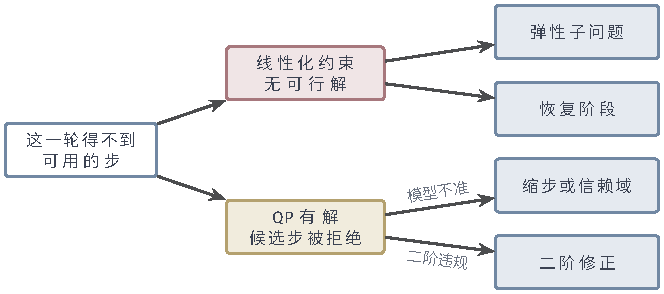
\includegraphics[width=112mm]{figures/05-optimization/06-constrained-optimization/tikz/sqp-repair-tree/figure.pdf}
 \caption{得不到可用的步时的两类原因及其修复。红框是子问题层面的失败，黄框是候选步层面的失败，蓝框是对应的处理。}
 \label{fig:sqp-repair-tree}
\end{BookInlineFigure}

\subsection{可行性恢复}
\label{sec:sqp-restoration}

\paragraph{线性化约束可能相互矛盾}
原问题可行，并不意味着它的线性化可行。看下面的问题：
\begin{equation}
 \min_{\bm{x}}\ \frac12\bigl((x_1-2)^2+x_2^2\bigr)
 \quad\text{s.t.}\quad h_1=x_2-x_1^2=0,\quad h_2=x_2-1=0.
 \label{eq:sqp-inconsistent}
\end{equation}
可行点只有$(\pm1,1)^\top$，解是$\bm{x}^\star=(1,1)^\top$。从原点出发，约束的值和Jacobian是
\[
 \bm{h}^{(0)}=(0,-1)^\top,\qquad\bm{A}^{(0)}=\begin{bmatrix}0&1\\0&1\end{bmatrix}.
\]

线性化约束成为$d_2=0$和$d_2=1$，两者矛盾。抛物线在顶点的切线是水平的，与直线$x_2=1$平行，图~\ref{fig:sqp-inconsistent}(a)里两条线永不相交。这里$\bm{A}^{(0)}$的秩为$1$，定理~\ref{thm:sqp-eqp}的前提失效。

\begin{BookInlineFigure}
 \centering
 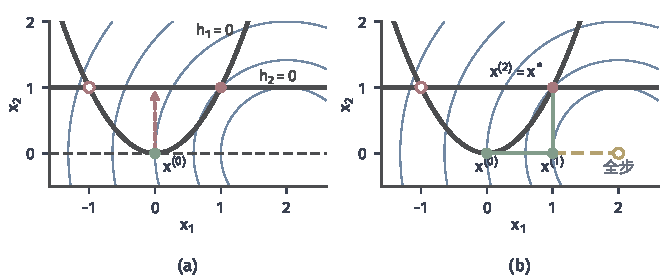
\includegraphics[width=112mm]{figures/05-optimization/06-constrained-optimization/matplotlib/sqp-inconsistent/figure.pdf}
 \caption{问题~\eqref{eq:sqp-inconsistent}。深灰粗线是抛物线$h_1=0$和直线$h_2=0$，蓝线是目标的等高线，红点是解，空心点是另一个可行点。(a)~原点处抛物线的线性化（虚线）与$h_2=0$平行，红色箭头表示两者之间的距离无法消除。(b)~弹性子问题的全步到$(2,0)^\top$（黄色虚线），回溯到一半得$\bm{x}^{(1)}$，下一轮的QP相容，一步到解。}
 \label{fig:sqp-inconsistent}
\end{BookInlineFigure}

\paragraph{弹性子问题}
第一种修复是让约束可以有偿违反。给每条线性化约束加上非负的松弛变量，并在目标中按权重$\rho$收费，得到\term{弹性子问题}（elastic subproblem）：
\begin{equation}
 \begin{aligned}
 \min_{\bm{d},\bm{v},\bm{w},\bm{u}}\quad & \langle\nabla f,\bm{d}\rangle+\frac12\bm{d}^\top\bm{B}\bm{d}
 +\rho\bigl(\langle\bm{1},\bm{v}+\bm{w}\rangle+\langle\bm{1},\bm{u}\rangle\bigr)\\
 \text{s.t.}\quad & \bm{h}+\bm{A}\bm{d}=\bm{v}-\bm{w},\\
 & \bm{g}+\bm{G}\bm{d}\leq\bm{u},\\
 & \bm{v},\bm{w},\bm{u}\geq\bm{0}.
 \end{aligned}
 \label{eq:sqp-elastic}
\end{equation}
它对任何数据都可行，取$\bm{d}=\bm{0}$，松弛变量等于当前的违反量即可。

消去松弛变量，式~\eqref{eq:sqp-elastic}就是在线性化约束上最小化$\ell_1$惩罚的模型。第~\ref{chap:penalty-multiplier-methods}章的精确惩罚论证用在这个凸QP上，得到：当线性化约束相容且$\rho$大于QP乘子的最大绝对值时，松弛变量全为零，弹性解就是原来QP的解。所以可以总是求解弹性形式，不必先判断QP是否可行。

例中取$\bm{B}^{(0)}=\bm{I}$，$\rho=1$。$\nabla f=(-2,0)^\top$，消去松弛变量后，模型是
\[
 -2d_1+\frac12d_1^2+\frac12d_2^2+\lvert d_2\rvert+\lvert d_2-1\rvert.
\]

对$d_1$的最小化独立于$d_2$，得$d_1=2$。在$0\leq d_2\leq1$上两个绝对值之和恒为$1$，这个区间内只剩$\frac12d_2^2$起作用，所以$d_2=0$。于是
\[
 \bm{d}^{(0)}=(2,\ 0)^\top,\qquad\text{模型中的违反量}=1.
\]

这一步并没有修好$h_2$，只是把目标朝$x_1$方向推。候选点要用真实函数检验。起点的评价函数是$\phi_1(\bm{0})=2+1=3$，全步的值和半步的值分别是
\[
 \phi_1(2,0)=0+4+1=5,\qquad\phi_1(1,0)=0.5+1+1=2.5.
\]

全步因线性化高估而被拒绝，半步通过。于是$\bm{x}^{(1)}=(1,0)^\top$。这里$h_1=-1$，梯度变成$(-2,1)$，第一行不再与第二行平行，线性化约束变成
\[
 -1-2d_1+d_2=0,\qquad-1+d_2=0.
\]

它有唯一解$\bm{d}^{(1)}=(0,1)^\top$，下一点恰好就是$(1,1)^\top$。这里能一步到解有偶然的成分，两个约束两个变量，线性化解恰好落在抛物线上。要点是离开奇异点之后，线性化又恢复了相容，图~\ref{fig:sqp-inconsistent}(b)是这条路径。

\paragraph{恢复阶段}
第二种修复更彻底。暂时不管$f$，改而求解只关心可行性的问题：
\begin{equation}
 \min_{\bm{x}}\ \theta(\bm{x}).
 \label{eq:sqp-restoration}
\end{equation}
这称为\term{可行性恢复}（feasibility restoration）。当回溯到很小的步长仍不被过滤器或评价函数接受，或者弹性子问题的松弛变量长期不为零时，就转入恢复阶段。

恢复阶段的目标与原优化目标不同，这是必须记住的。它不保证目标下降，甚至可能把目标抬得很高。一旦违反量明显减小，并且新点能被过滤器接受或线性化重新相容，就停止恢复，在新点重建SQP模型，回到原来的目标上。

\paragraph{恢复失败说明不了什么}
恢复阶段可能停在$\theta$的局部最小点，而$\theta$在那里仍然为正。这能证明原问题无可行解吗？不能。看单变量约束
\[
 h(x)=x^3-3x+3=0.
\]

$h'(x)=3x^2-3$在$x=1$处为零，且$h(1)=1>0$，所以$x=1$是$\lvert h\rvert$的局部最小点。从$x=1$附近出发的恢复过程会困在这里，而方程在$x\approx-2.104$有实根。局部方法看到的只是局部信息，它只能报告“在这里找不到可行点”，要证明不可行需要全局的论证或对偶证书。

\subsection{二阶修正（补充）}
\label{sec:sqp-soc}

第~\ref{sec:sqp-merit}小节留下一个疑点：好的全步被评价函数拒绝。本小节要回答的问题是：这种误判从何而来，怎样在不放弃这个步的前提下消除它？

\paragraph{好步被拒绝}
下面的问题是弯曲约束上的典型例子：
\begin{equation}
 \min_{\bm{x}}\ 2(x_1^2+x_2^2-1)-x_1
 \quad\text{s.t.}\quad h=x_1^2+x_2^2-1=0.
 \label{eq:sqp-maratos}
\end{equation}
解是$\bm{x}^\star=(1,0)^\top$，在此处驻定条件$(3,0)^\top+\nu(2,0)^\top=\bm{0}$给出$\nu^\star=-3/2$。取$\nu=\nu^\star$，于是$\bm{B}=(4+2\nu)\bm{I}=\bm{I}$。

取圆上的点$\bm{x}=(0.8,0.6)^\top$，此时$h=0$，$f=-0.8$，梯度和Jacobian是
\[
 \nabla f=(2.2,\ 2.4)^\top,\qquad\bm{A}=(1.6,\ 1.2).
\]

解KKT系统。用$\bm{A}$左乘第一行并用$\bm{A}\bm{d}=0$，由$\bm{A}\nabla f=6.4$和$\bm{A}\bm{A}^\top=4$得$\hat\nu=-1.6$，于是
\[
 \bm{d}=(0.36,\ -0.48)^\top,\qquad\bm{x}+\bm{d}=(1.16,\ 0.12)^\top.
\]

这一步很好：到解的距离从$0.632$缩短到$0.2$。可是真实函数值都变差了：
\[
 f(\bm{x}+\bm{d})=-0.44>-0.8,\qquad h(\bm{x}+\bm{d})=0.36>0.
\]

目标上升，违反量也上升，对任何$\rho>0$，$\phi_\rho$都升高了，这一步被拒绝。过滤器同样拒绝，因为记录$(0,-0.8)$在两个指标上都压过候选$(0.36,-0.44)$。这种现象称为\term{Maratos效应}（Maratos effect）：全步本可带来快速的局部收敛，却被接受规则判为失败，迫使算法缩短步长，收敛变慢。

原因在于约束的弯曲。线性化保证$\bm{A}\bm{d}=-\bm{h}$，但二阶项留在了约束上，$h(\bm{x}+\bm{d})=\lVert\bm{d}\rVert_2^2=0.36$。这个二阶大小的违反，足以抵消模型预期的目标下降。Lagrange函数其实是下降的，目标的增量$0.36$加上$\nu^\star$乘约束的增量$0.36$，合计是$-0.18$。评价函数中$\ell_1$项的绝对值把这一点丢掉了。

\paragraph{补一个修正步}
既然问题是二阶的违反，就补一步把它修掉。在$\bm{x}+\bm{d}$处重新计算约束的值，但沿用当前的Jacobian，求一个最小范数的修正：
\begin{equation}
 \hat{\bm{d}}=-\bm{A}^\top\bigl(\bm{A}\bm{A}^\top\bigr)^{-1}\bm{h}(\bm{x}+\bm{d}).
 \label{eq:sqp-soc}
\end{equation}
然后用$\bm{x}+\bm{d}+\hat{\bm{d}}$作候选点，这称为\term{二阶修正}（second-order correction）。

例中$\bm{A}\bm{A}^\top=4$，$h(\bm{x}+\bm{d})=0.36$，代入式~\eqref{eq:sqp-soc}，得
\[
 \hat{\bm{d}}=-(1.6,\ 1.2)^\top\times0.09=(-0.144,\ -0.108)^\top.
\]

修正后的候选点及其函数值是
\[
 \bm{x}+\bm{d}+\hat{\bm{d}}=(1.016,\ 0.012)^\top,\quad h=0.0324,\quad f=-0.9512.
\]

现在$\rho=2$时评价函数的值是$-0.9512+0.0648=-0.8864$，低于$-0.8$，步被接受，到解的距离只有$0.02$。过滤器也接受它，因为目标已满足$-0.9512\leq-0.8$。图~\ref{fig:sqp-maratos}(a)是这两段，(b)是整个迭代的比较。

\begin{BookInlineFigure}
 \centering
 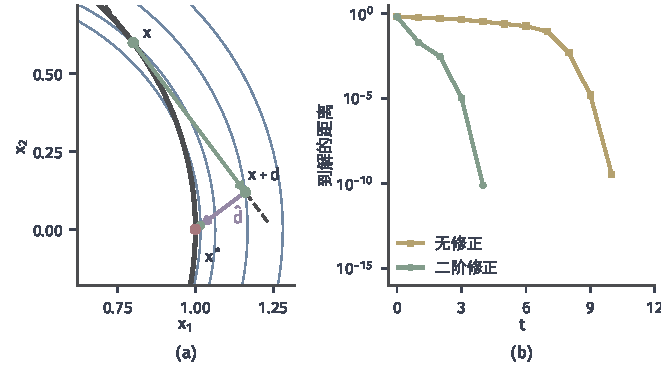
\includegraphics[width=112mm]{figures/05-optimization/06-constrained-optimization/matplotlib/sqp-maratos/figure.pdf}
 \caption{问题~\eqref{eq:sqp-maratos}上的Maratos效应与二阶修正。(a)~深灰粗线是约束，蓝线是目标的等高线，虚线是线性化约束；绿色箭头是QP步，紫色箭头是修正步$\hat{\bm{d}}$，红点是解。(b)~$\rho=2$、$\eta=0.1$的回溯SQP：不修正（黄）前七轮步长被缩短，修正（绿）后每轮都走全步。}
 \label{fig:sqp-maratos}
\end{BookInlineFigure}

\paragraph{为什么修正是二阶的}
设$\lVert\bm{d}\rVert_2$很小。约束在$\bm{x}+\bm{d}$处的值只剩二阶项，所以$\hat{\bm{d}}$的长度是$\lVert\bm{d}\rVert_2^2$的量级，比主步小一阶，不会破坏主步带来的快速收敛。

把修正后的点代入约束展开，$\bm{A}(\bm{x}+\bm{d})$与$\bm{A}(\bm{x})$之差是$\lVert\bm{d}\rVert_2$的量级，乘以$\hat{\bm{d}}$得三阶项；其余项也是三阶以上，因此修正后的违反量降到$\lVert\bm{d}\rVert_2^3$的量级。

\paragraph{与重新解QP的区别}
修正步用的是已有的$\bm{A}$和它的分解，只换了右端，代价是一次回代加一次约束求值。重新构造并求解QP则要重新求导和分解。有不等式时，修正要在主步的工作集上做，或者把线性化约束的常数项换成$\bm{g}(\bm{x}+\bm{d})-\bm{G}\bm{d}$再解一次QP，后者花费更多，但结果仍是原QP的一次扰动。

实现中通常只在全步被拒绝、且约束违反确实增加时才试一次修正，试探失败就回到回溯。也有别的办法绕开Maratos效应，例如暂时放行一步、几步之后再回头检查的非单调策略，以及改用可微的评价函数。
